\documentclass[10pt]{article}
\usepackage[T1]{fontenc}
\usepackage[utf8]{inputenc}
\usepackage[italian]{babel}
\usepackage{multicol}
\usepackage[a4paper, total={18cm, 25cm}]{geometry}
\usepackage{amsfonts}
\usepackage{lmodern}
\usepackage{graphicx}
\graphicspath{ {./img/} }

\begin{document}
{\fontfamily{lmss}\selectfont
\title{World Quizzle -- Relazione del progetto}
\author{Federico Matteoni -- Mat. 530257}
\date{ }
\renewcommand*\contentsname{Indice}

\maketitle
\section{Introduzione}
\paragraph{Funzionalità} Il progetto richiedeva lo sviluppo di \textbf{WordQuizzle}: un sistema di sfide di traduzione italiano--inglese tra gli utenti registrati al servizio.\\
Era richiesta la possibilità, per gli utenti registrati, di poter sfidare gli utenti appartenenti alla propria rete sociale di amicizie. Le sfide consistevano nella traduzione, nel minor tempo possibile, di una serie di parole italiane proposte dal servizio.
\paragraph{Architettura} Si richiedeva che l'applicazione fosse implementata secondo un'architettura client--server, con i componenti che comunicano \texttt{TCP}, \texttt{UDP} e tramite il meccanismo \texttt{RMI}. Inoltre si richiedeva, per il server, la persistenza delle informazioni degli utenti su un file \texttt{JSON}, e la richiesta delle traduzioni delle parole scelte ad un servizio esterno tramite richieste \texttt{HTTP GET}.\\
L'interazione con l'utente poteva avvenire tramite una \texttt{CLI} oppure, opzionalmente, una \texttt{GUI}. Per sperimentazione e sfida personale ho scelto la seconda.
\section{Overview del sistema}
Il sistema è suddiviso in due parti principali: \textbf{client} e \textbf{server}. Tramite il client è possibile interagire col servizio WordQuizzle, che viene offerto dal server.\\
L'\textbf{interfaccia del server} offre varie \textbf{informazioni sullo stato attuale del servizio}, dagli utenti alla porta usata. Può essere usata per verificare il corretto funzionamento del sistema e monitorare le sfide in corso.\\
L'\textbf{interfaccia del client} è usata per l'\textbf{interazione vera e propria} col servizio: da essa si possono lanciare le sfide, richiedere le informazioni al server e consultare la propria lista amici e lo stato del proprio profilo utente.
\subsection{Istruzioni per l'installazione e l'avvio}
\paragraph{Server} Il server, eseguito dall'archivio \texttt{WordQuizzleServer.jar}, \textbf{deve trovarsi in una directory contenente il dizionario} da cui selezionare le parole per la sfida. Il dizionario contiene \texttt{N} parole italiane, una per riga. Un dizionario di esempio con 100 parole è incluso.\\
Per avviare il server, è sufficiente eseguirlo con il comando \texttt{java -jar WordQuizzleServer.jar <porta>}, passando il numero di porta su cui stabilire le connessioni con il parametro \texttt{<porta>}.
\paragraph{Client} Il client viene eseguito a partire dall'archivio \texttt{WordQuizzleClient.jar} tramite il comando\\\texttt{java -jar WordQuizzleClient.jar <porta>}, specificando la porta del server a cui collegarsi tramite il parametro \texttt{<porta>}.
\pagebreak
\subsection{Server}
\begin{center}
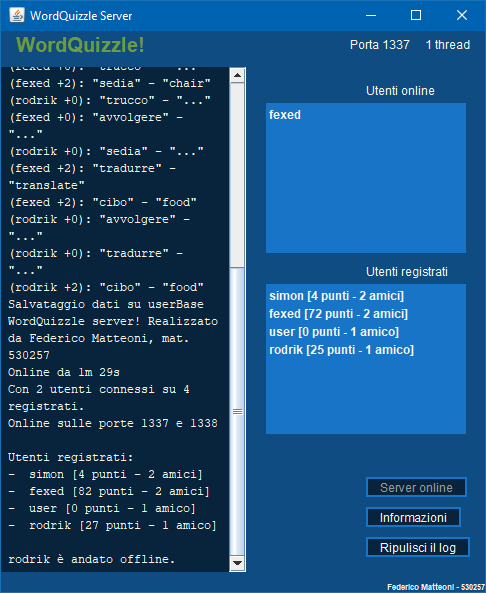
\includegraphics[scale=0.75]{server.png}
\end{center}
\paragraph{Interfaccia} L'interfaccia del server è strutturata in modo da fornire a colpo d'occhio informazioni utili quali: utenti online e registrati, eventi recenti del servizio come sfide, connessioni e disconnessioni.\\
L'interfaccia cerca di essere il più chiara e intuitiva possibile: sulla sinistra si trova il log del servizio, mentre sulla destra sono elencati gli utenti online, quelli registrati e i comandi per avviare il server, stampare delle informazioni utili sul log o ripulirlo. In alto sono indicati il numero di porta su cui il server ascolta le connessioni in arrivo e il numero di thread attualmente eseguiti dal server.\\
La scritta "WordQuizzle" in alto a sinistra viene colorata di rosso o di verde a seconda dello stato in cui si trova il server, rispettivamente offline od online.
\paragraph{Funzionalità} Il server si avvia automaticamente al lancio dell'eseguibile, ascoltando sul numero di porta specificato. Può essere chiuso come una qualsiasi applicazione dalla \texttt{X} in alto a destra sulla barra del titolo della finestra. In caso di errori ed eccezioni, il server stamperà i messaggi di errore sullo standard output (solitamente, la console da dove è stato lanciato) per poter verificare il messaggio dell'errore che si è verificato.\\
Quanto al servizio WordQuizzle, è possibile fare doppio click su un utente registrato per poter verificare le sue informazioni quali nome utente, password e punteggio, oltre alle amicizie nel dettaglio.
\begin{center}
Le informazioni di un utente\\
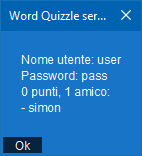
\includegraphics[scale=1]{infouser.png}
\end{center}
\pagebreak
\subsection{Client}
\begin{center}
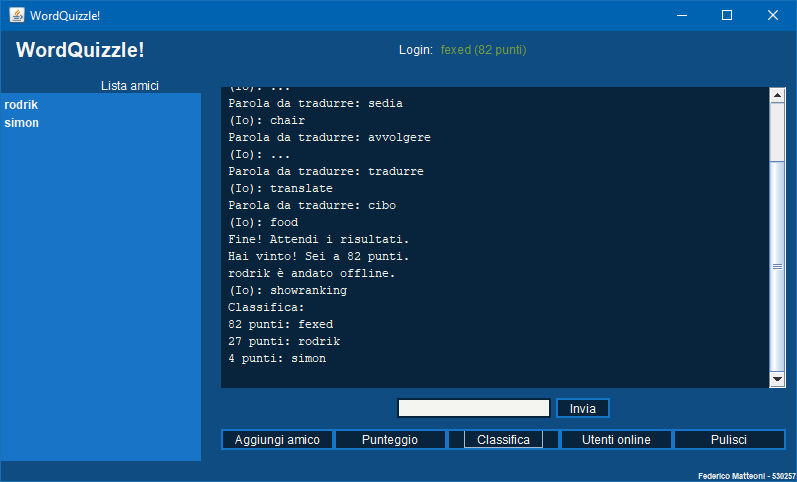
\includegraphics[scale=0.75]{client.png}
\end{center}
\paragraph{Interfaccia} L'interfaccia dell'utente è pensata per essere facilmente fruibile in modo da ottenere le informazioni necessarie dal server o sfidare rapidamente un utente della propria lista amici. La finestra presenta al centro il log dei messaggi spediti e ricevuti dal server, mentre sulla sinistra c'è la lista amici dell'utente connesso. Le informazioni dell'utente sono visibili in alto, con punteggio e nome utente colorato di verde o rosso a seconda se il client è, rispettivamente, connesso o meno.\\
In basso si trova la barra di testo in cui inserire i comandi o, durante una sfida, le traduzioni proposte. Il pulsante "\texttt{Invia}" è selezionabile anche con il tasto \texttt{Invio} della tastiera, per permettere allo sfidante di rispondere il più velocemente possibile durante la sfida di traduzione. I pulsanti inferiori mandano dei messaggi che il server interpreta come richiesta di informazioni.\\
Il pulsante "\texttt{Aggiungi amico}" apre una finestra di dialogo che richiede il nickname dell'utente da aggiungere.\\
La finestra di \textbf{login} si apre automaticamente all'avvio del client, mentre in caso di caduta della connessione e client offline apparirà un pulsante "\texttt{Login}" a destra del punteggio, per poter reinstaurare la connessione.
\paragraph{Funzionalità} Per poter \textbf{sfidare un amico} è sufficiente fare doppio click sul nome utente dell'amico che si vuole sfidare. Il sistema gestirà la richiesta e la risposta: una finestra di dialogo apparirà sul client dell'amico che si vuole sfidare e attenderà una risposta per 10s. In caso di risposta affermativa, la sfida partirà per entrambi gli utenti.\\
L'aggiunta di un amico, la richiesta di punteggio, classifica e utenti online sono tutte funzionalità richiedibili tramite gli appositi pulsanti nella parte inferiore dell'interfaccia.\\
Eventuali errori che richiedono attenzione sono visualizzati come finestra di dialogo contenente il messaggio d'errore.
\begin{multicols}{2}
\begin{center}
La finestra di login\\
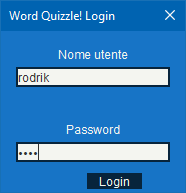
\includegraphics[scale=1]{login.png}
\end{center}
\begin{center}
La richiesta di sfida\\

\includegraphics[scale=1]{sfida.png}
\end{center}
\end{multicols}
\pagebreak

}
\end{document}